\documentclass{beamer}
\usetheme{metropolis}
\usepackage{graphicx}
\usepackage{subfig}
\usepackage{tcolorbox}
\title{Calculus-Based Physics-2: Electricity and Magnetism (PHYS180-02): Unit 2}
\author{Jordan Hanson}
\institute{Whittier College Department of Physics and Astronomy}

\begin{document}
\maketitle

\section{Unit 1 Review}

\begin{frame}{Unit 1 Summary}
\textbf{Reading: Chapters 5-6}
\begin{enumerate}
\item Charge, Conductors and Insulators
\item Coulomb's Law and Electric Fields
\item E-fields of Charge Distributions
\item Gauss's Law
\end{enumerate}
\end{frame}

\section{Unit 1 Review Problems}

\begin{frame}{Unit 3 Review Problems}
Suppose a charge $q$ is located at the origin.  Use Gauss' law to find the electric field.  What is the electric field?
\begin{itemize}
\item A: $\vec{E} = \frac{kq}{r}\hat{r}$
\item B: $\vec{E} = \frac{kq}{r^2}\hat{r}$
\item C: $\vec{E} = \frac{kq}{r^3}\hat{r}$
\item D: $\vec{E} = \frac{kq^2}{r^2}\hat{r}$
\end{itemize}
\end{frame}

\begin{frame}{Unit 3 Review Problems}
Suppose a line of charge runs up the z-axis.  The charge per unit length is $\lambda$.  Use Gauss' law to find the electric field.  What is the electric field at a point $P = (x,0,0)$?
\begin{itemize}
\item A: $\vec{E} = \frac{2k\lambda}{r^2} \hat{x}$
\item B: $\vec{E} = \frac{2k\lambda^2}{r^2} \hat{x}$
\item C: $\vec{E} = \frac{2k\lambda}{r} \hat{x}$
\item D: $\vec{E} = 0$
\end{itemize}
\end{frame}

\section{Summary}

\begin{frame}{Unit 4 Summary}
\textbf{Reading: Chapters 7-8}
\begin{enumerate}
\item Voltage
\begin{enumerate}
\item Review of work and energy
\item Review of conservative forces
\end{enumerate}
\item Capacitance
\end{enumerate}
\end{frame}

\section{Voltage}

\begin{frame}{Voltage}
\alert{Voltage} is analogous to potential energy in electrostatics.  The negative derivative of potential energy U is the force F:
\begin{equation}
F = -\frac{dU}{dx}
\end{equation}
For example, if the force is $F = -mg$, and the potential energy is $U = mgy$, then 
\begin{equation}
\frac{dU}{dy} = -mg
\end{equation}
\end{frame}

\begin{frame}{Voltage}
\alert{Voltage} is analogous to potential energy in electrostatics.  The derivative of voltage V is the field E:
\begin{equation}
E = -\frac{dV}{dx}
\end{equation}
For example, if the field is $E = \sigma/\epsilon_0$, and the potential energy is $V = \sigma/\epsilon_0 x + C$, then 
\begin{equation}
\frac{dV}{dx} = \sigma/\epsilon_0
\end{equation}
\end{frame}

\begin{frame}{Voltage}
\alert{Voltage} is analogous to potential energy in electrostatics. \\ \vspace{1cm}
Potential energy is just an energy.  A \textit{potential} in mechanics is the potential energy per unit mass.  \textit{Voltage}, or \textit{electrostatic potential} is \textbf{\alert{potential energy per unit charge.}} \\ \vspace{0.5cm}
The Volt (V) is the unit of voltage, and it has units of 1 V = 1 J/C.
\end{frame}

\begin{frame}{Voltage}
\textbf{Group board exercise}: Show that the units of electric field (normally Newtons per Coulomb) are also Volts per meter.
\end{frame}

\begin{frame}{Voltage}
\small
If the potential energy is a function of displacement, $U = U(\vec{x})$, it may be called a potential energy \textit{surface}.
\begin{figure}
\centering
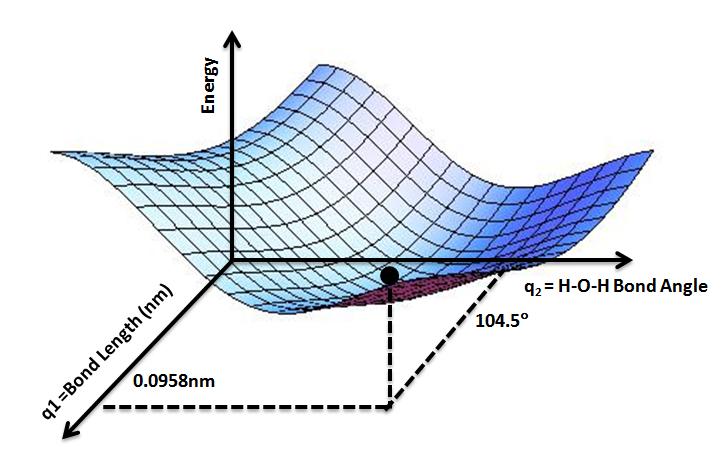
\includegraphics[width=0.5\textwidth]{figures/potential.png}
\caption{\label{fig:potential} An example of a potential energy surface.}
\end{figure}
\end{frame}

\begin{frame}{Voltage}
\small
Considering \textit{Newton's Second Law}, however, if $F = m a$ then $m a = -\frac{\Delta U}{\Delta x}$, and
\begin{equation}
a = -\frac{1}{m}\frac{\Delta U}{\Delta x} \label{eq:field}
\end{equation}
\begin{figure}
\centering
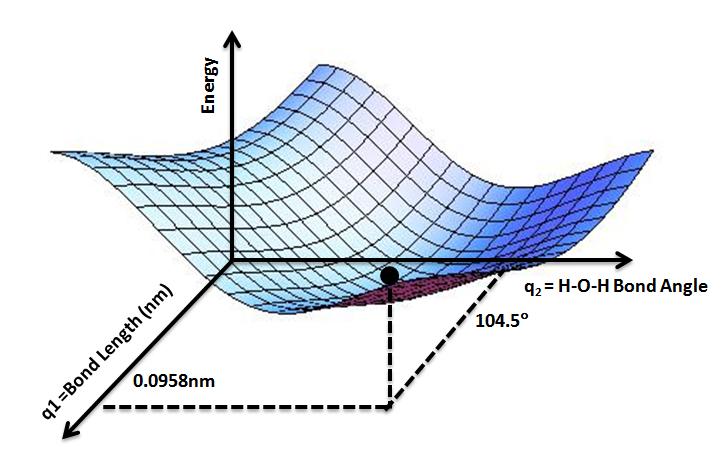
\includegraphics[width=0.4\textwidth]{figures/potential.png}
\caption{\label{fig:potential2} If we divide by the mass we have acceleration.}
\end{figure}
The derivative, or \textit{gradient}, of $a$ in Eq. \ref{eq:field} is analogous to the electric field.  But the electric field is a \textit{vector field}...
\end{frame}

\begin{frame}{Voltage}
The gradient is like a derivative, but gives you the proper direction wherever you are.
\begin{equation}
\boxed{
-\vec{\nabla} V = \vec{E} = -\frac{\partial V}{\partial x}\hat{i}-\frac{\partial V}{\partial y}\hat{j}-\frac{\partial V}{\partial z}\hat{k}}
\end{equation}
\end{frame}

\begin{frame}{Unit 3 Review Problems}
Suppose the voltage due to some charge distribution is $V(x,y,z) = ax+b$.  What is the field?
\begin{itemize}
\item A: $\vec{E} = a\hat{j}$
\item B: $\vec{E} = a\hat{k}$
\item C: $\vec{E} = b\hat{i}$
\item D: $\vec{E} = -a\hat{i}$
\end{itemize}
\end{frame}

\begin{frame}{Unit 3 Review Problems}
Suppose the voltage due to some charge distribution is $V(x,y,z) = ax+by$.  What is the field?
\begin{itemize}
\item A: $\vec{E} = -a\hat{j}-b\hat{j}$
\item B: $\vec{E} = a\hat{k}+b\hat{k}$
\item C: $\vec{E} = -b\hat{i}-a\hat{j}$
\item D: $\vec{E} = -a\hat{i}-b\hat{j}$
\end{itemize}
\end{frame}

\begin{frame}{Voltage}
Suppose a charge distribution is made of two infinite plates of charge with charge per unit area $\pm\sigma$.  We know that the field is $\sigma/\epsilon_0 \hat{k}$ between them.  \textbf{Group board exercise}: Draw the charge distribution, define a coordinate system, and write the function for the voltage.
\end{frame}

\begin{frame}{Voltage}
\textbf{Voltage} is like a potential energy surface $\rightarrow$ \textit{potential energy per unit charge.} \\ \vspace{0.5cm}
\url{https://phet.colorado.edu/en/simulation/charges-and-fields} \\
\alert{Using the PhET simulation about charges and fields}:
\begin{enumerate}
\item Explore the voltage associated with fields generated by charges using the voltage button.
\item Add a single point charge, and use the ruler and voltmeter (potentiometer) to measure voltage versus distance, and plot it.
\item What function describes the relationship between voltage and distance?
\end{enumerate}
\end{frame}

\begin{frame}{Voltage}
\url{https://phet.colorado.edu/en/simulation/charges-and-fields} \\
\alert{Using the PhET simulation about charges and fields}:
\begin{enumerate}
\item Note that the units of $\epsilon_0$ are N m$^2$ C$^{-2}$, and the value is $8.854\times 10^{-12}$
\item We know from prior equations that the units of voltage are J C$^{-1}$
\item Using your measurements, show that the voltage due to a point charge is
\begin{equation}
\boxed{
V = \pm \frac{1}{4\pi \epsilon_0} \frac{q}{r}}
\end{equation}
(Where the sign depends on the charge, just like E-fields)
\end{enumerate}
\end{frame}

\begin{frame}{Voltage}
Voltage due to a point charge:
\begin{equation}
\boxed{
V = \pm \frac{1}{4\pi \epsilon_0} \frac{q}{r}} \label{eq:volt2}
\end{equation}
\end{frame}

\begin{frame}{Voltage}
Voltage is an example of a \textbf{scalar field}, whereas the electric field is an example of a \textbf{vector field.}  Create two lines of charge, one positive and one negative in the PHeT simulator, and pretend they represent planes of charge coming out of the screen.  The field should constant and uniform like
\begin{equation}
\vec{E} = \frac{\sigma}{\epsilon_0} \hat{k}
\end{equation}
\begin{enumerate}
\item Plot the voltage versus distance between the plates.
\item Calculate the slope in V/m, and the y-intercept in V.
\item Does the electric field depend on the y-intercept?  Does the charge distribution?
\end{enumerate}
\end{frame}

\begin{frame}{Voltage}
\begin{figure}
\centering
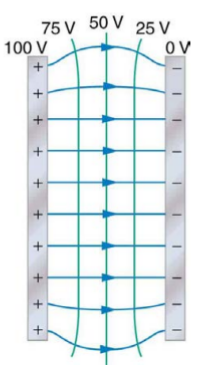
\includegraphics[width=0.25\textwidth]{figures/plates.png}
\caption{\label{fig:plates} Parallel plates of charge, electric field, and potential.  Notice the linear decrease in voltage.}
\end{figure}
\textbf{How we define the y-intercept in voltage is analogous to the zero-point freedom of potential energy.}
\end{frame}

\begin{frame}{Voltage}
\textit{Two parallel plates, opposite charge}:
\begin{equation}
V = -\frac{\sigma}{\epsilon_0}z + C
\end{equation}
With the boundary condition that $V = V_0$ when $z = 0$, we have
\begin{equation}
V(z) - V_0 = -\frac{\sigma}{\epsilon_0}z
\end{equation}
Let $\Delta V(z) = V(z) - V_0$, and $\Delta z = z$:
\begin{equation}
-\frac{\Delta V}{\Delta z} = \frac{\sigma}{\epsilon_0} =  E
\end{equation}
\end{frame}

\begin{frame}{Voltage}
\textbf{Continuing with PHeT:} Make a ring of charge that has a radius of 100 cm, with the center at the origin.
\begin{enumerate}
\item Show that the voltage field is radially symmetric.
\begin{itemize}
\item Place \textit{equipotential lines} around the charge distribution and see that they are circular.
\end{itemize}
\item Show that at distances much larger than the radius, the voltage field looks like that of a point charge.
\begin{itemize}
\item Record the voltage versus distance from the origin.
\item Plot the data.
\item Compare to the plot corresponding to a point charge.
\end{itemize}
\end{enumerate} 
\end{frame}

\section{Units of Energy}

\begin{frame}{Units of Energy}
The electron-volt: eV.  This is the energy gained by an electron accelerated through a voltage of 1 V.
\begin{itemize}
\item How many Joules per electron volt?
\item What is the mass of a proton in eV? (E = mc$^2$, where $c$ is the speed of light.)
\end{itemize}
\end{frame}

\begin{frame}{Units of Energy}
A proton is released into a 40 kV electric potential.  What is the final kinetic energy of the proton?
\begin{itemize}
\item A: -20 kV
\item B: 40 kV
\item C: -40 keV
\item D: 40 keV
\end{itemize}
\end{frame}

\begin{frame}{Units of Energy}
An alpha particle is a helium nucleus with a charge of $+2 q_e$.  Suppose an alpha particle is accelerated and has a final energy of 2 MeV.  How many volts were required to accelerated it?
\begin{itemize}
\item A: 4 MV
\item B: 3 MV
\item C: 2 MV
\item D: 1 MV
\end{itemize}
\end{frame}

\begin{frame}{Units of Energy}
\begin{figure}
\centering
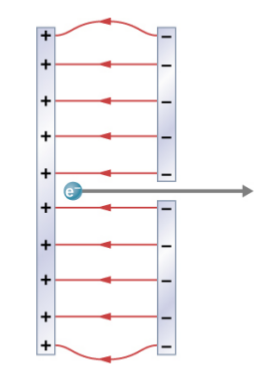
\includegraphics[width=0.3\textwidth]{figures/accel_plates.png}
\caption{\label{fig:accel_plate} An electron accelerated by a parallel plate capacitor.}
\end{figure}
\end{frame}

\begin{frame}{Units of Energy}
An electron has a charge $-q_e$.  Suppose an electron is accelerated through a voltage of 1 V toward another electron at a fixed position.  How close does the moving electron get to the stationary one?
\begin{itemize}
\item A: about 0.1 nm
\item B: about 1 nm
\item C: about 10 nm
\item D: about 100 nm
\end{itemize}
\end{frame}

\begin{frame}{Units of Energy}
A bare helium nucleus has two positive charges and a mass of $6.64 \times 10^{-27}$ kg.  What is the kinetic energy at 2 percent of the speed of light?  The speed of light is $c = 3.0 \times 10^{8}$ m/s.
\begin{itemize}
\item A: $1.2 \times 10^{-10}$ J
\item B: $1.2 \times 10^{-11}$ J
\item C: $1.2 \times 10^{-12}$ J
\item D: $1.2 \times 10^{-13}$ J
\end{itemize}
\end{frame}

\begin{frame}{Units of Energy}
What is the previous energy in eV?
\begin{itemize}
\item A: 0.75 MeV
\item B: 0.75 keV
\item C: 0.75 GeV
\item D: 0.75 eV
\end{itemize}
\end{frame}

\begin{frame}{Units of Energy}
Remember that this is an alpha particle (helium nucleus) with a +2 charge.  How many volts are required to give it an energy of 0.75 MeV?
\begin{itemize}
\item A: 0.375 MV
\item B: 0.75 MV
\item C: 1.5 MV
\item D: 0.375 V
\end{itemize}
\end{frame}

\section{Capacitance}

\begin{frame}{Capacitance}
\textbf{Capacitance} is the ability of an object to store charge.  Let the voltage difference across an object be $V$, storing $-Q$ on one side and $+Q$ on another.  The \textit{capacitance} $C$ is given by
\begin{equation}
Q = C V
\end{equation}
Let the object be two parallel plates, and the charges be $\pm Q$.
\end{frame}

\begin{frame}{Capacitance}
\begin{figure}
\centering
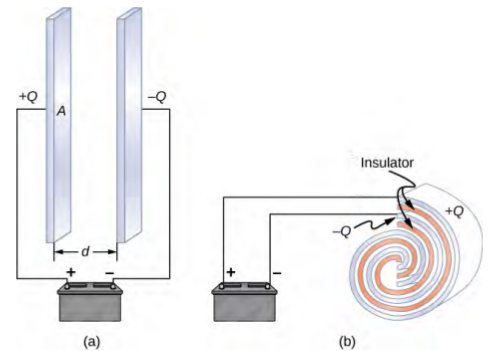
\includegraphics[width=0.8\textwidth]{figures/cap.png}
\caption{\label{fig:cap} General scheme of a capacitor.}
\end{figure}
\end{frame}

\begin{frame}{Capacitance}
The electric field and voltage between two charged plates separated by a distance $d$ is $V = Ed$.  The field is $E = \sigma/\epsilon_0$, and $Q = \sigma/A$, where $A$ is the plate area and $\sigma$ is the surface charged density.  Note that
\begin{align}
C = Q/V &= (Q)/(E d) \\
= (Q \epsilon_0)/(\sigma d) &= (Q A \epsilon_0)/(Q d) \\
= \frac{A \epsilon_0}{d} &
\end{align}
So the capacitance depends on the permittivity of free space, the area, and the distance.  In other words, just the geometry of the system.  The units of capcitance are \textbf{\alert{Farads}} (F).  This is a large unit.  Typical capacitors have nF or pF.
\end{frame}

\begin{frame}{Capacitance}
\textbf{Group board exercise}: The permittivity of free space is $8.85 \times 10^{-12}$ N$^{-1}$ C$^2$ m$^{-2}$.  A capacitor has an area of 1 mm$^2$, and $d = 0.001$ mm.  What is the capacitance? \\ 
\textbf{Group board exercise}: The permittivity of free space is $8.85 \times 10^{-12}$ N$^{-1}$ C$^2$ m$^{-2}$.  A capacitor has an area of 10 mm$^2$, and $d = 0.001$ mm.  What is the capacitance? \\
\textbf{Group board exercise}: The permittivity of free space is $8.85 \times 10^{-12}$ N$^{-1}$ C$^2$ m$^{-2}$.  A capacitor has an area of 1 mm$^2$, and $d = 0.01$ mm.  What is the capacitance?
\end{frame}

\section{Capacitors in series and in parallel}

\begin{frame}{Capacitors in series and in parallel}
\textbf{Observe on board.}
\begin{enumerate}
\item Consider two capacitors \textit{in series,} with capacitance $C_1$ and $C_2$.  What is the total capacitance?
\item Consider two capacitors \textit{in parallel,} with capacitance $C_1$ and $C_2$.  What is the total capacitance?
\end{enumerate}
\textbf{Create a simple circuit with capacitors}, and a battery to charge them.  How much total charge is stored?  Exchange your design with another group, and solve each others' problem.
\end{frame}

\section{The Cylindrical Capacitor and Coaxial Cables}

\begin{frame}{The Cylindrical Capacitor and Coaxial Cables}
\begin{figure}
\centering
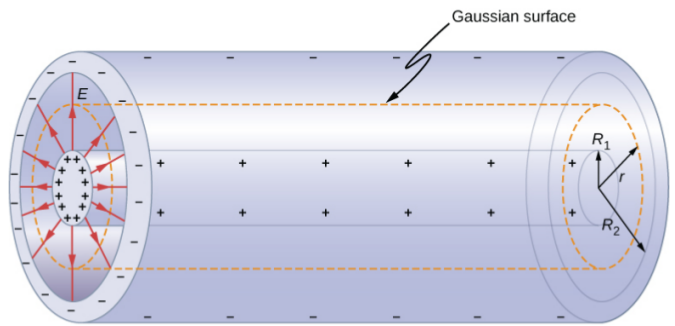
\includegraphics[width=0.7\textwidth]{figures/cyl.png}
\caption{\label{fig:cyl} A cylindrical capacitor, as a model for a coaxial cable.  There is an inner radius and an outer radius, with our Gaussian surface drawn in between the two conductors.}
\end{figure}
\end{frame}

\begin{frame}{The Cylindrical Capacitor and Coaxial Cables}
Recall that
\begin{align}
Q &= \Delta VC \\
\Delta V &= - \int_{R_1}^{R_2} \vec{E} \cdot d\vec{r}
\end{align}
\begin{itemize}
\item What is the electric field $\vec{E}$ of a section of this coaxial cable of length $l$? (\textit{Recall from warm-up.}).
\item What if we integrate from positive charge (inner radius) to negative charge (outer)? \textbf{Observe on board.}
\end{itemize}
\end{frame}

\begin{frame}{The Cylindrical Capacitor and Coaxial Cables}
Thus we have the capacitance per unit length:
\begin{equation}
\boxed{
\frac{C}{l} = \frac{2\pi\epsilon_0}{\ln(R_2/R_1)}
}
\end{equation}
What are the units of $\epsilon_0$?
\begin{itemize}
\item A: F/m$^2$
\item B: F/m
\item C: F/$\ln(m)$
\item D: F
\end{itemize}
\end{frame}

\begin{frame}{The Cylindrical Capacitor and Coaxial Cables}
Thus we have the capacitance per unit length:
\begin{equation}
\boxed{
\frac{C}{l} = \frac{2\pi\epsilon_0}{\ln(R_2/R_1)}
}
\end{equation}
Suppose the cap per unit length is 0.1 nF, and we \textit{square} $R_2/R_1$.  What is the new cap per unit length?
\begin{itemize}
\item A: 0.1 nF
\item B: 0.05 nF
\item C: 0.2 nF
\item D: 0 nF
\end{itemize}
\end{frame}

\begin{frame}{The Cylindrical Capacitor and Coaxial Cables}
Thus we have the capacitance per unit length:
\begin{equation}
\boxed{
\frac{C}{l} = \frac{2\pi\epsilon_0}{\ln(R_2/R_1)}
}
\end{equation}
Suppose the cap per unit length is 0.1 nF, and we \textit{triple} $\epsilon_0$ in some way.  What is the new cap per unit length?
\begin{itemize}
\item A: 0.1 nF
\item B: 0.2 nF
\item C: 0.3 nF
\item D: 0.5 nF
\end{itemize}
\end{frame}

\begin{frame}{The Cylindrical Capacitor and Coaxial Cables}
(Preview of Unit 3).  Suppose we have a system that obeys
\begin{equation}
v(t) = R \frac{dQ}{dt} = i(t) R
\end{equation}
This is called \textbf{Ohm's law.}
\begin{figure}
\centering
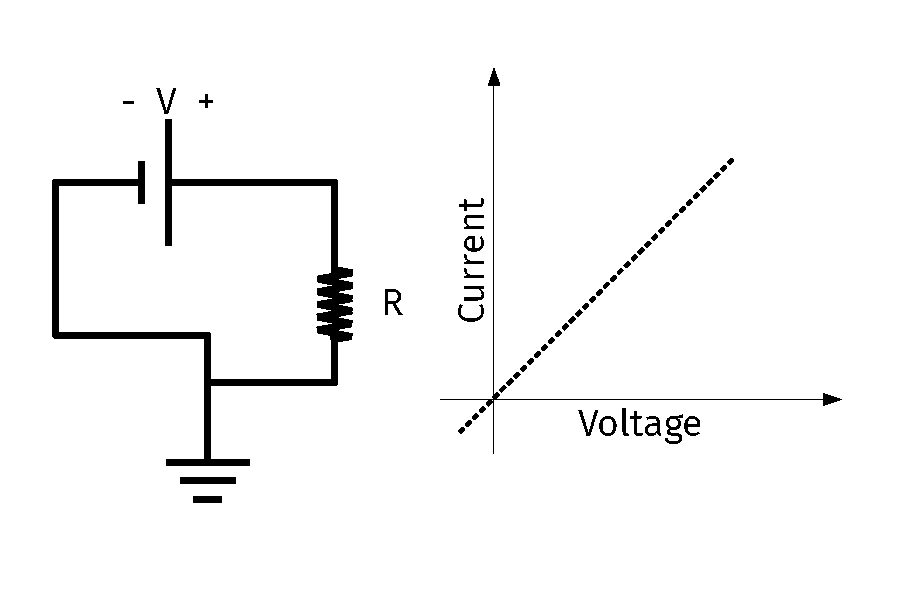
\includegraphics[width=0.55\textwidth]{figures/iVCurve.pdf}
\caption{\label{fig:iv} A simple circuit with a resistor element, some voltage, and \textit{ground.} This just means that 0V is at the negative terminal.}
\end{figure}
\end{frame}

\begin{frame}{The Cylindrical Capacitor and Coaxial Cables}
(Preview of Unit 3).  What if we add a capacitor?
\begin{equation}
V_0 = R \frac{dQ}{dt} +\frac{Q}{C}
\end{equation}
This is called \textbf{Ohm's law.}
\begin{figure}
\centering
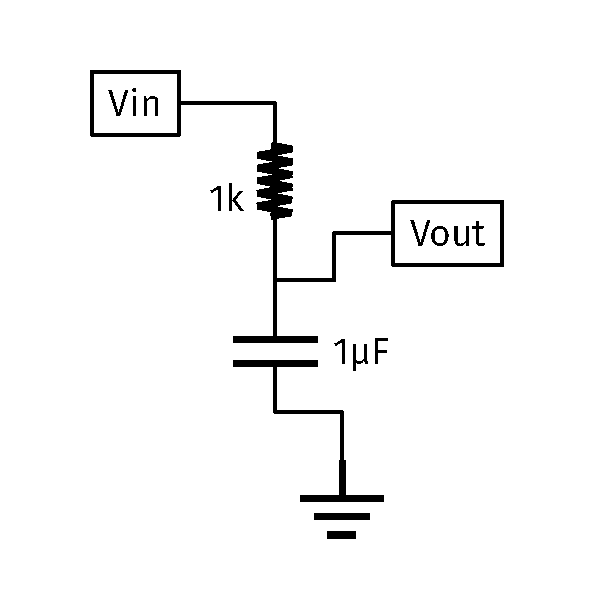
\includegraphics[width=0.45\textwidth]{figures/iVCurve8.pdf}
\caption{\label{fig:iv2} A simple circuit with a resistor and capacitor elements.}
\end{figure}
\end{frame}

\begin{frame}{The Cylindrical Capacitor and Coaxial Cables}
(Preview of Unit 3).  What if we add a capacitor?
We can show that
\begin{equation}
V_{out}(t) = V_0 \exp(-t/\tau)
\end{equation}
with $\tau = RC$.  Thus, if we send a signal $V_{in}$ down a ``very long'' coaxial cable, with some capacitance per unit length, it will not exit the cable. \\ \vspace{0.5cm}
For example: \url{https://www.pasternack.com/images/ProductPDF/LMR-400.pdf} \\ \vspace{0.5cm}
What is the attenuation per 100 m of this cable at 150 MHz?
\end{frame}

\section{Conclusion}

\begin{frame}{Unit 4 Summary}
\textbf{Reading: Chapters 7-8}
\begin{enumerate}
\item Voltage
\begin{enumerate}
\item Review of work and energy
\item Review of conservative forces
\end{enumerate}
\item Capacitance
\end{enumerate}
\end{frame}

\section{Answers}

\begin{frame}{Answers}
\small
\begin{columns}[T]
\begin{column}{0.5\textwidth}
\begin{itemize}
\item $\vec{E} = \frac{kq}{r^2}\hat{r}$
\item $\vec{E} = \frac{2k\lambda}{r}$
\item $\vec{E} = -a\hat{i}$
\item $\vec{E} = -a\hat{i}-b\hat{j}$
\item 40 keV
\item 1 MV
\item about 1 nm
\item $1.2 \times 10^{-13}$ J
\item 0.75 MeV
\item 0.375 MV
\end{itemize}
\end{column}
\begin{column}{0.5\textwidth}
\begin{itemize}
\item F/m
\item 0.05 nF
\item 0.3 nF
\end{itemize}
\end{column}
\end{columns}
\end{frame}

\end{document}
